\subsection{Nonsupercritical, T3-like, and Vd1/Vd2 Reach Branches}
\label{sec:t3-vd-demand-branches}

\subsubsection{The exactly-one-$T3$ branch}

\begin{proposition}[Exactly one T3-like V triangle]
\label{prop:nplus-one-one-t3}
Assume the C triangle is CE1 or CE2, $N_+=1$, exactly one V triangle is
T3-like, no triangle is Vd1 or Vd2, and $N_{\mathrm{gap}}\ge1$.  Then the
triangles do not cover $H$.
\end{proposition}

\begin{proof}
By Proposition~\ref{prop:unique-center-midpoint}, normalize so that
$T_C\cap\{M_0,\ldots,M_5\}=\{M_0\}$.  A T3-like V triangle misses its own
midpoint, a supercritical V triangle misses its local midpoint, and an
open role $U_i$ whose closure $T_i$ is Vd0 cannot contain $M_{i-1}$ or
$M_{i+1}$.
Consequently, after reflection,
\[
 T_0\text{ is T3-like},\qquad M_1\in T_0,
 \qquad T_1\text{ is uniquely supercritical},
\]
and $T_2,\ldots,T_5$ are nonsupercritical Vd0 V triangles.  The rational local
calculation is Lemma~\ref{lem:short-t3-rescuer-profile}.  It verifies the two
local inequalities in \eqref{eq:signed-rescuer-local}, while midpoint and
support isolation force the center to cover the $O$-side radial gap.  The
common adjacent-exception obstruction, Corollary~\ref{cor:signed-adjacent-rescuers},
therefore gives the contradiction.
\end{proof}

\subsubsection{The nonsupercritical CE1/CE2 boundary packages}

Figure~\ref{fig:ce1-ce2-n0-all-vd0} gives a common schematic for the package
proved below.

\begin{figure}[H]
\centering
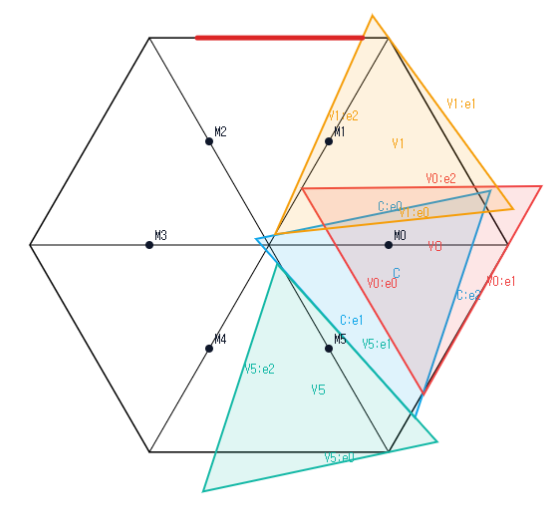
\includegraphics[width=.78\linewidth]
  {figures/strategy2_ce1_ce2_n0_all_vd0.png}
\caption{Schematic view of the common CE1/CE2, $N_+=0$, all-Vd0 boundary
package, not to scale.  The C triangle and three representative Vd0 vertex
triangles are shown; the remaining three triangles are omitted for readability.  The
simultaneous placement is not a candidate cover, and no proof depends on
visual inspection.}
\label{fig:ce1-ce2-n0-all-vd0}
\end{figure}

\begin{proposition}[Nonzero-gap all-Vd0 skeleton-data obstruction]
\label{prop:nplus-zero-all-vd0}
Let the C triangle be CE1 or CE2. Assume all six V triangles are Vd0,
\[
 A_i+B_i\le1\qquad(i=0,\ldots,5),
\]
the seven open triangles cover the full skeleton
\[
 S=\partial H\cup\bigcup_{i=0}^5r_i,
\]
and assume $N_{\mathrm{gap}}\ge1$.  Then no such configuration exists; in
particular, these data cannot cover all of $H$.
\end{proposition}

\begin{proof}
Let $d_i^C$ be the center reach on $r_i$, measured from $O$, and set
$c_i^C=1-d_i^C$. Since every V triangle is Vd0,
$\Haus(T_{i-1}\cap r_i)=\Haus(T_{i+1}\cap r_i)=0$; diameter locality
excludes every $T_j$ with $j\notin\{i-1,i,i+1\}$.
Skeleton coverage therefore forces
\[
 C_i\ge c_i^C\qquad(i=0,\ldots,5).
\tag{\(*\)}
\]

Let $N_{\mathrm{gap}}$ be the number of positive center traces containing a
boundary gap. Singleton boundary gaps are included. By hypothesis and the
center classification, $N_{\mathrm{gap}}\in\{1,2\}$, with
$N_{\mathrm{gap}}=1$ in CE1.

Suppose $N_{\mathrm{gap}}=1$. Normalize the active trace to
\[
 I_R=\left[\frac{k}{R},W+\delta\right]\subset e_{0,1}
\]
and put
\[
 s=\frac{k}{R},\qquad q=R-\delta.
\]
Gap containment gives $B_0\ge s$ and $A_1\ge q$. The companion edge is
absent or gap-free, so $A_0+B_5\ge1$; since $A_0+B_0\le1$, one has
$B_5\ge s$. By \((*)\),
\[
 C_1\ge1-\frac\delta R,
 \qquad
 C_5\ge1-\frac\alpha W.
\]
The exact one-side endpoint theorem gives
\[
 M_{1-\alpha/W}(s)
 +M_{1-\delta/R}(q)<1.
\]
The three internal V triangles $T_2,T_3,T_4$ lie on a center-free boundary
path. The path budget forces their total boundary contribution above three,
contrary to their three nonsupercritical caps.

If $N_{\mathrm{gap}}=2$, the center is CE2. The paired endpoint theorem, together
with \((*)\), gives
\[
 p=W-\alpha,\qquad q=R-\delta,
 \qquad \overline M_{p/W}(p)+\overline M_{q/R}(q)<1.
\]
The same center-free three-V triangle path gives the contradiction.

The two nonzero gap ranks are exhaustive.
\end{proof}

We next treat the additional T3-like V triangles in the $N_+=0$ branch.  The
following local facts also reappear later.

\begin{lemma}[T3-like midpoint and side tradeoff]
\label{lem:t3-midpoint-tradeoff}
Let $T_i$ be T3-like.  Then $M_i\notin T_i$.  After applying the closed-trace
domination of Proposition~\ref{prop:t3-translation}, suppose
$\Haus(T_i\cap r_{i+1})>0$ and $M_{i+1}$ belongs to the dominated trace.
If $b$ is its boundary reach toward $V_{i+1}$, $c$ its exit on $r_i$, and
$\ell$ its entry on $r_{i+1}$, all measured from the relevant
vertex, then
\begin{equation}
 b+c<1,\qquad b+\ell>1.
 \label{eq:t3-side-tradeoff}
\end{equation}
Consequently two T3-like traces $T_i,T_{i+1}$ that cover each other's
midpoint, with positive traces on $r_{i+1}$ and $r_i$, respectively, cannot
cover both segments $[V_i,M_i]$ and $[V_{i+1},M_{i+1}]$ if no other triangle
has positive trace there.
\end{lemma}

\begin{proof}
Apply Proposition~\ref{prop:t3-translation} and reflect if necessary.  Its
translated Type-II majorant has parameters
\[
 0<t<1,\qquad z=\sqrt{1-t+t^2},\qquad \alpha=0,\qquad 0<\beta<z.
\]
Its wedge vertex has
\[
 Q_x=\frac{z-t\beta}{1-t+t^2}>1.
\]
Hence
\[
 t\beta<z-z^2.
\]
The majorant's radial exit is $c=\beta/(1-t)$.  Since
\[
 (1-z)(1+z)=t(1-t),
\]
we obtain
\[
 c<\frac{z-z^2}{t(1-t)}=\frac{z}{1+z}<\frac12.
\]
Here $z<1$ because $0<t<1$.  Thus the translated majorant misses $M_0$,
and its closed-trace domination
implies that the original T3-like triangle misses $M_0$ as well.

For the tradeoff, the translated T3-like trace has the exhaustive Type-II
form
\[
 \begin{aligned}
 (1-t)x+ty&\ge0,\\
 \beta+tx-y&\ge0,\\
 \beta+x-(1-t)y&\le z,
 \end{aligned}
 \qquad 0<t<1,\quad z=\sqrt{1-t+t^2},\quad0<\beta<z.
\]
For the selected support on $r_1$, substitution in the Type-II half-planes
gives
\[
 b=z-\beta,\qquad c=\frac{\beta}{1-t},\qquad
 \ell=\frac{\beta+1-z}{1-t}.
\]
The condition $M_1\in T$ is
$\beta\le z-(1+t)/2$.  Therefore
\[
 b+c\le z+\frac{t}{1-t}
 \left(z-\frac{1+t}{2}\right)
 =1-\frac{(1-z)^2}{2(1-t)}<1,
\]
whereas
\[
 b+\ell-1=\frac{t(1-z+\beta)}{1-t}>0.
\]
For a crossed adjacent pair, write $(b,c,\ell)$ for the first triangle's
boundary reach, own-arm exit, and opposite-arm entry, and write
$(\widetilde b,\widetilde c,\widetilde\ell)$ for the reflected quantities of
the second.  Equation~\eqref{eq:t3-side-tradeoff} and its reflection give
\[
 b+c<1,\quad b+\ell>1,\qquad
 \widetilde b+\widetilde c<1,\quad
 \widetilde b+\widetilde\ell>1.
\]
Coverage forces $c\ge\widetilde\ell$ and
$\widetilde c\ge\ell$.  The first inequality gives
$\widetilde b+c>1>b+c$, hence $\widetilde b>b$; the second gives
$b+\widetilde c>1>\widetilde b+\widetilde c$, hence
$b>\widetilde b$, a contradiction.
\end{proof}

\begin{lemma}[The support-isolated four-branch inequality]
\label{lem:407-four-label-loss}
\label{thm:s2-geom-t3}
Assume the support-isolated T3-like endpoint state of
Definition~\ref{def:body-t3-endpoint-state}.  Then the two endpoint V triangles
satisfy
\begin{equation}
 \overline M_{c_5^\ast}(a_5^\ast)+\overline M_{c_1^\ast}(a_1^\ast)<1,
 \label{eq:407-loss}
\end{equation}
where $a_1^\ast,a_5^\ast$ are the exact boundary inputs and
$c_1^\ast,c_5^\ast$ the exact radial lower bounds defined there.
\end{lemma}

\begin{proof}
Use the CE1 side variables $0<\lambda<1$,
$\rho=\sqrt{1-\lambda+\lambda^2}$ and center slacks
\[
 X=F_0(O),\qquad Y=F_2(O).
\]
Then
\[
 a_C=\lambda-Y,\qquad
 \lambda s=X+Y+1-\rho,
\]
and Proposition~\ref{prop:signed-center-normal-form} gives
\[
 \rho-X-Y>\frac12,\qquad
 \frac Y\lambda<\frac12,\qquad
 \frac X{1-\lambda}<\frac12.
\]
Consequently the apparent minima in the two radial exits collapse to
\[
 \gamma_1=\frac Y\lambda,\qquad
 \gamma_5=\frac X{1-\lambda}.
\]
For CE2 the second boundary interval is $[S,T]$, where
\[
 S=\frac{X+Y+1-\rho}{1-\lambda},\qquad T=X+\lambda.
\]

The T3-like normal form supplies $D>1$, $0<R<1$, and $\alpha,p\ge0$ with
\[
 R^2-DR+D^2=1,\qquad \alpha+p=1/D,\qquad
 q=1-p=\alpha+(D-1)/D<1/2.
\]
Its interval on $r_1$, measured from $V_1$, is
\[
 [c,u],\qquad c=Dq/R,\qquad u=q+(1-R)/D.
\]
Using the residual operator \eqref{eq:reader-residual-operator}, the exact
boundary inputs are, with $J_1=[s,t]$ and with $J_5=[S,T]$ in CE2 but
$J_5=\varnothing$ in CE1,
\[
 a_1^\ast=\mathcal R_{J_1}(p),\qquad
 a_5^\ast=\mathcal R_{J_5}(\alpha),
\]
and
\[
 c_5^\ast=1-\gamma_5,\qquad
 c_1^\ast=
 \begin{cases}
 c,&1-u\le\gamma_1\le1-c,\\
 1-\gamma_1,&\text{otherwise}.
 \end{cases}
\]

If $a_1^\ast+a_5^\ast>1$, the two caps already imply
$\overline M_{c_5^\ast}(a_5^\ast)+\overline M_{c_1^\ast}(a_1^\ast)<1$.  Assume the hard region
$a_1^\ast+a_5^\ast\le1$.  The following table is an exhaustive case analysis of the four
possible first branches; the middle column states the exact decisive
inequality.
\[
\begin{array}{c|c|c}
\text{first branch}&\text{right branches}&\text{conclusion}\\ \hline
\mathrm{Const}&\mathrm{Lin}&e(\gamma_5)<a_1^\ast\\
\mathrm{Const}&\mathrm{Const},Q_-&\overline M_{c_5^\ast}(a_5^\ast)+\overline M_{c_1^\ast}(a_1^\ast)<1\\
\mathrm{Const}&Q_+&e(\gamma_5)<a_1^\ast\\
Q_-&\mathrm{Const},Q_-&\overline M_{c_5^\ast}(a_5^\ast)+\overline M_{c_1^\ast}(a_1^\ast)<1\\
Q_-&\mathrm{Lin},Q_+&\overline M_{c_5^\ast}(a_5^\ast)<a_1^\ast\\
\mathrm{Lin}&\text{all}&\text{impossible}\\
Q_+&\mathrm{Lin},Q_+&\text{impossible}\\
Q_+&\mathrm{Const},Q_-&\overline M_{c_5^\ast}(a_5^\ast)+\overline M_{c_1^\ast}(a_1^\ast)<1.
\end{array}
\]
We verify the nonformal entries.  Put
$\kappa=(1-\rho)/(1-\lambda)$.  From
$X+(1-\lambda)Y<\rho(1-\rho)$ one obtains
\begin{align}
 \gamma_1\ge a_C&\Longrightarrow e(\gamma_5)<a_C,
 \label{eq:407-core-estimate}\\
 S\le Y/\lambda&\Longrightarrow e(\gamma_5)<S.
 \label{eq:407-S-estimate}
\end{align}
For \eqref{eq:407-core-estimate}, one has
$\gamma_5<a_C-\kappa$ and
$a_C-\kappa<1/8$; then \eqref{eq:low-root-bounds} applies, and the remaining
comparison is
\[
 (a_C-\kappa)+5(a_C-\kappa)^2\le\kappa.
\]
After squaring its positive sides, the difference is
$\lambda(23\lambda^3+58\lambda^2+7\lambda+72)>0$.
For \eqref{eq:407-S-estimate}, combine the premise with the center
inequality and put $x=\lambda$.  This gives $0<x<3/8$ and
\[
 X<X_*=\frac{(1-\rho)(\rho(1-2x)-x(1-x))}{1-x-x^2}.
\]
Set
\[
 \delta=\frac{1-\rho}{1-x}=\frac{x}{1+\rho},\qquad
 \eta=\frac{X}{1-x},\qquad
 f=\rho(1-2x)-x(1-x),\qquad d=1-x-x^2.
\]
Then $\gamma_5\le\eta<\delta f/d$.  Moreover
\[
 \frac fd<1-2x,
\]
because, after multiplication by positive denominators, this is just
\[
 \rho<d+\frac{x(1-x)}{1-2x}
 =1+\frac{2x^3}{1-2x}.
\]
Hence $\eta<\delta(1-2x)<1/8$.  If $\eta=0$, the assertion is immediate.
Otherwise,
\[
 S\ge\frac{X+1-\rho}{1-2x}
 =\frac{1-x}{1-2x}(\eta+\delta)
 >2\eta\left(\frac{1-x}{1-2x}\right)^2.
\]
On the other hand,
\[
 5\eta<5\delta(1-2x)
 <2\left[\left(\frac{1-x}{1-2x}\right)^2-1\right].
\]
For the middle sign use $\rho>1-x$ and
\[
2(2-3x)(2-x)-5(1-2x)^3
 =(4x-3)(10x^2-6x-1)>0
 \qquad(0<x<3/8).
\]
Indeed both factors are negative; for the quadratic use
$10x^2\le15x/4<6x+1$.
The low-root estimate \eqref{eq:low-root-bounds} now gives
\[
 e(\gamma_5)\le2\gamma_5+5\gamma_5^2
 \le2\eta+5\eta^2<S,
\]
proving \eqref{eq:407-S-estimate} without any polynomial coefficient list.
The constant-branch separation follows from its exact polynomial: if its output is
$z=e(\eta)$ at input $1-\beta$, then
\[
 \beta\ge z+\eta.
 \label{eq:407-L-separation}
\]
Indeed the selector polynomial
$P(x,z)=x^4-4x^3+5x^2-(2+z)x+z-z^2$ is strictly decreasing on the low
range and vanishes at $x=\eta$.  Equations
\eqref{eq:407-core-estimate}--\eqref{eq:407-L-separation}, with the three
residual cases in $\mathcal R_J$, prove every first-constant entry.  For a first $Q_-$
branch the exact root test
\[
 Q_-(a,c)<z\iff c^2(a+z)^2-(a^2-ac+c^2)>0
\]
is increasing in $z$.  Substitution of $a_1^\ast$, followed by the center
inequality, proves $\overline M_{c_5^\ast}(a_5^\ast)<a_1^\ast$ except in the low--low entries, which
are immediate from $Q_-(a,c)\le\min\{a,1-a\}$ and the constant-branch output is below $1/2$.
First-coordinate linear would force either
$X\ge(1-\lambda)\alpha$ and $Y\ge\lambda-\alpha$, contradicting
$s\le p$, or, in the CE2 overlap case, $S\ge1/2$, contradicting
$S\le\alpha<1/2$.

For a first $Q_+$ branch put $r=1-\lambda$,
$y=Y/\lambda$ and choose $\beta$ so that
\[
 m=\sqrt{\beta^2-\beta+1},\quad
 1-\gamma_5=\frac m{r+\beta},\quad
 \overline M_{c_5^\ast}(a_5^\ast)=\frac{\beta m}{r+\beta}.
\]
The exact selector is
\begin{equation}
 \beta\ge\max\left\{r,\frac12,\frac{1-r^2}{1+2r}\right\},\qquad
 r\ge(1-\beta)(r+\beta)^2.
 \label{eq:407-high-domain}
\end{equation}
The center inequalities give $y<1/10$ and, with
\[
 y_*=\frac r{1-r}
 \left(\frac m{r+\beta}-\frac12-\frac{1-r}{1+\sqrt{r^2-r+1}}\right),
\]
give $y<y_*$ and
\[
 3y_*\le1-\frac{\beta m}{r+\beta}.
\]
This proves the right-constant entry by $e(y)<3y$.  It excludes right linear and
right high by the exact high-input filter.  For right $Q_-$ with input
$a_C$, direct substitution gives a sum below one.  For input $q$, put
$c=1-y$, $q=tc$, and let $\widehat b_1=\overline M_{c_1^\ast}(q)$.  The selected $Q_-$ equations
give
\[
 \widehat b_1\le\kappa:=\frac{\sqrt{13}-1}{6},\qquad
 q\le\tau<\frac{93}{200},
\]
where $\tau\in(0,1/2)$ is the unique root of
$\tau^4-3\tau^3+3\tau^2-3\tau+1=0$.  In this CE2 overlap subcase the
support ordering gives $q>S$.  The common left-high identities are
\[
 S=S_0+\frac{1-r}{r}y,\qquad
 S_0=1-\frac{m}{r+\beta}+\frac{1-r}{1+\sqrt{r^2-r+1}}.
\]
Since $y>0$, we have the complete chain
\[
 S_0<S<q\le\tau<\frac{93}{200}.
\]
We now replace the former interval subdivision by a one-variable comparison.
Write $s=r+\beta$ and $\rho_r=\sqrt{r^2-r+1}$.  The selected Cell~2
inequality factors as
\[
 r-(1-\beta)(r+\beta)^2
 =(s-1)(\beta^2+r\beta-r).
\]
The second factor is nonnegative because $r\le\beta$ and $\beta\ge1/2$;
if it vanishes, then $r=\beta=1/2$.  Hence $s\ge1$.  It follows that
$\rho_r\le m$, since
$\rho_r^2-m^2=(r-\beta)(s-1)\le0$.

Define the one-variable lower bound
\[
 \overline S(\beta)=1-m+\frac{\beta}{1+m}.
\]
Then
\[
 S_0\ge1-\frac m s+\frac{1-r}{1+m}\ge\overline S(\beta).
\]
Indeed, the second difference is
\[
 (s-1)\left(\frac m s-\frac1{1+m}\right)\ge0.
\]
For the last sign use $s\le2\beta\le m(1+m)$: if
$\gamma_\beta=3\beta-\beta^2-1$, then $\gamma_\beta>0$ and
\[
 m^2-\gamma_\beta^2=-\beta(\beta-1)(\beta^2-5\beta+5)\ge0,
 \qquad m^2+\gamma_\beta=2\beta.
\]

Put $\beta_0=5657/10000$, $T=93/200$, and $\beta_*=161/250$.
If $\beta m/s\ge\beta_0$, then $\beta m\ge\beta_0$. The function
$\phi(\beta)=\beta m$ is strictly increasing, and the exact comparison
\[
 \beta_0^2-\beta_*^2m(\beta_*)^2
 =\frac{22782769}{62500000000}>0
\]
therefore gives $\beta>\beta_*$.  On $[\beta_*,1]$ put
\[
 \chi(\beta)=\frac{107}{200}-Tm-(1-\beta)^2.
\]
Since $\chi''=-3T/(4m^3)-2<0$, the function $\chi$ is concave. Its endpoint
values are positive: $\chi(1)=7/100$, while, for
$a_*=107/200-(1-\beta_*)^2=51033/125000$,
\[
 a_*^2-T^2m(\beta_*)^2
 =\frac{1693881}{62500000000}>0.
\]
Thus $\chi>0$ throughout the interval. The identity
\[
 (\overline S(\beta)-T)(1+m)=\chi(\beta)
\]
shows that $\beta m/s\ge\beta_0$ would force $S_0>T$, a contradiction.
Consequently
\[
 \overline M_{c_5^\ast}(a_5^\ast)<\frac{5657}{10000}
 <\frac{7-\sqrt{13}}6.
\]
The final strict comparison follows by squaring
$\sqrt{13}<18029/5000$, whose squared difference is
$44841/25000000>0$.
Thus the final sum is also below one.  The table is exhaustive, proving
\eqref{eq:407-loss}.
\end{proof}

\begin{proposition}[The nonzero-gap $N_+=0$ T3-like branch]
\label{prop:nplus-zero-t3}
Assume that $T_C$ is CE1 or CE2, $N_+=0$, no V triangle is Vd1 or Vd2,
at least one V triangle is T3-like, and $N_{\mathrm{gap}}\ge1$.  Then the
seven triangles do not cover $H$.
\end{proposition}

\begin{proof}
By Proposition~\ref{prop:unique-center-midpoint}, normalize so that
$T_C\cap\{M_0,\ldots,M_5\}=\{M_0\}$, and simultaneously apply the
closed-trace domination of Proposition~\ref{prop:t3-translation} to every
T3-like triangle.  If $T_0$ were not T3-like, a maximal consecutive block of
T3-like indices among $1,\ldots,5$ would have to match its triangles bijectively
to the same block of uncovered midpoints.  Each match sends $T_i$ only to
$M_{i-1}$ or $M_{i+1}$, because a T3-like triangle misses $M_i$ and an
open role $U_i$ whose closure $T_i$ is Vd0 cannot contain $M_{i-1}$ or
$M_{i+1}$.
Its first two triangles therefore form a crossed pair
forbidden by Lemma~\ref{lem:t3-midpoint-tradeoff}.  Hence $T_0$ is T3-like;
reflect so that $\Haus(T_0\cap r_1)>0$.

There are at most two T3-like triangles. Indeed, with $N_+=0$ and no
Vd1/Vd2 triangle, their number $k$ equals $N_{\mathrm{sp}}$. If $k\ge3$,
Theorem~\ref{thm:common-skeleton-count} gives an immediate full-skeleton
contradiction.
Midpoint locality then forces $T_2,T_4,T_5$ to be Vd0.  Consequently $r_1$
has positive support only from $T_C,T_0,T_1$, and $r_5$ only from $T_C,T_5$.

Thus all hypotheses of the support-isolated state in
Definition~\ref{def:body-t3-endpoint-state} hold.  The actual forward reaches
of $T_1,T_5$ are bounded by the two safe maps in
Lemma~\ref{lem:407-four-label-loss}; an extra reach lower bound on $r_0$ or
$r_2$ for a possible T3-like $T_1$ only shrinks its feasible set.  Thus their sum is
less than one.  V triangles $T_2,T_3,T_4$ must cover more than three units of the
four intervening boundary edges, while their three nonsupercritical caps
sum to at most three.  This contradiction proves the proposition.
\end{proof}

\subsubsection{Two reusable high-radial endpoint inequalities}

\begin{lemma}[One-side endpoint loss]
\label{lem:one-side-capped-loss}
\label{thm:s2-geom-e1}
Let $0<R<1$, $S=\sqrt{1-R+R^2}$, and let $s,u,w>0$ satisfy
$s+u+w=1$ and $0<u<R$.  Put
\[
 \delta=\frac{R}{1+S},\qquad
 \gamma=u-\delta-\frac{R}{1-R}w,
\]
and assume $\gamma>0$.  Set
\[
 c_1=u/R,\qquad c_5=1-\gamma.
\]
Then
\begin{equation}
 \overline M_{c_5}(s)+\overline M_{c_1}(u)<1.
 \label{eq:one-side-loss}
\end{equation}
\end{lemma}

\begin{proof}
Put $\eta=(1-R)\delta=1-S$ and
\[
 \widehat b_5=\overline M_{c_5}(s),\qquad
 \widehat b_1=\overline M_{c_1}(u).
\]
The center identity may be written
\begin{equation}
 c_5=\frac{1-u+\eta-Rs}{1-R}.
 \label{eq:one-side-center-line}
\end{equation}
The hypotheses imply $1/2<c_1,c_5<1$: for example
$u>\delta$ gives $c_1>1/(1+S)>1/2$, and
$\gamma<u-\delta<R-\delta=RS/(1+S)<1/2$ gives $c_5>1/2$.
Thus the four high-radial branches of
the four-branch high-radial map in Proposition~\ref{prop:capped-demand-map} are exhaustive.

\smallskip\noindent
\emph{Right low branches.}
If the right branch is $Q_-$, its exact frontier equation gives
$(u+\widehat b_1)^2=1-R+R^2=S^2$, so $\widehat b_1=S-u$.  For a right constant branch write
$\widehat b_1=kc_1$, $0\le k\le1/2$, and $C=1-k+k^2=c_1^2$.  With $X_R=R+k$, the
constant-branch selector factors as
\[
 q=c_1^2(X_R-1)G_k(X_R),\qquad
 G_k(X)=CX^3+CX^2-k(1-k)X+k^2.
\]
For $X\ge k$, $G_k(X)>0$: when $k>0$,
$G_k'(X)\ge k(1+2k-k^2+3k^3)>0$ and
$G_k(k)=k^2(1+k+k^3)>0$.  Hence $q\le0$ gives $X_R\le1$.  If
$h_R=1-X_R$, then
\[
 S^2-(u+\widehat b_1)^2=h_R(1+2k^2+k(1-k)h_R)\ge0.
\]
Consequently either right low branch satisfies
\begin{equation}
 \widehat b_1\le X:=S-u.
 \label{eq:one-side-right-low}
\end{equation}

\smallskip\noindent
\emph{A left low branch against right high or linear.}
For left $Q_-$ put $z=s/c_5=1-p$ and
$h=\sqrt{1-p+p^2}$.  The component selector gives
$0\le p\le1/2$, the frontier gives $s+\widehat b_5=h$, and its selector gives
$s\le(1-p)h$.  Equation \eqref{eq:one-side-center-line} becomes
$c_5(1-Rp)=1-u+\eta$, whence
\[
 u\ge \eta+(1-h)+Rph.
\]
Put $q_0=ph$.  If $q_0>R$, then
$p(1-p)>R(1-R)$ and the preceding lower bound would give $u>R$.
Thus $q_0\le R$, and
\[
 \eta+1-h>
 \frac{R(1-R)+p(1-p)}2\ge(1-R)q_0.
\]
Substitution in the exact formula
\[
 w=\frac{(1-R)(1-u)p-\eta(1-p)}{1-Rp}
\]
now gives $w<1-h$. A right high output has the form $\omega_\beta-u$, where
$\omega_\beta=\sqrt{1-\beta+\beta^2}\le1$; for linear take
$\omega_\beta=1$. Hence
\[
 \widehat b_5+\widehat b_1=h+\omega_\beta-(s+u)
 =1+w-(1-h)-(1-\omega_\beta)<1.
\]

For a left constant branch write
\[
 c_5=h(x):=\sqrt{1-x+x^2},\qquad
 \widehat b_5=xh(x),\qquad 0\le x\le\frac12,
\]
and, along the center line,
\[
 s(x)=\frac{R-u+\eta+(1-R)(1-h(x))}{R}.
\]
If $y=s(x)/h(x)$, the exact selector factorization is
\[
 \frac{q}{h(x)^2}=(y-(1-x))P_x(y),
\]
where
\begin{align*}
 P_x(y)={}&(1-x+x^2)y^3+(1+2x-2x^2+3x^3)y^2\\
 &+(x+2x^2-x^3+3x^4)y+(x^2+x^3+x^5).
\end{align*}
Every coefficient is nonnegative on $0\le x\le1/2$, and the polynomial is
positive at every nondegenerate point.  Thus a selected constant-branch point has
$s(x)\le(1-x)h(x)$.  The two curves meet once in $(0,1/2)$: at $x=0$ the
left side is smaller, while at $x=1/2$ it is enough to use
\[
 u\le\frac{R}{1+R}\quad(\mathrm{Lin}),\qquad
 u\le\min\{RS,S/2\}\quad(Q_+).
\]
Writing $e_0=1-\sqrt3/2$, the corresponding endpoint differences are
\[
 \frac{(1-R)(R^2+2Re_0+2e_0)}{2(1+R)}>0
\]
for linear, and respectively
$[2e_0(1-R)-R^3]/2\ge0$ for $R\le1/2$ and
$(1-R)(3R+4e_0-2)/4\ge0$ for $R\ge1/2$ in the high case.
At the unique transition $x_0$, the constant frontier is the $q=0$ endpoint of
the preceding $Q_-$ branch.  Since $xh(x)$ increases, every selected left constant-branch output is no larger than that transition output.  The preceding strict
loss therefore also covers $(\mathrm{Const},Q_+)$ and $(\mathrm{Const},\mathrm{Lin})$.

\smallskip\noindent
\emph{linear and high exclusions.}
Left linear forces $s<1/2$ and $\gamma\ge s$.  Right linear or right high gives
$u\le1/2$, but
\[
 \gamma-s=2u-1-\delta+\frac{1-2R}{1-R}w<0:
\]
for $R\ge1/2$ this is immediate, while for $R<1/2$ use $w<1-u$ to bound it
by $(u-R)/(1-R)-\delta<0$.  Thus left linear cannot pair with either branch.
If the left branch is high and the right one linear, then $s<1/2$ and
$u\le R/(1+R)$, whereas $\gamma>0$ and $w>1/2-u$ force
$u>R/2+\eta>R/(1+R)$; the final inequality is equivalent to
$2(1+R)>1+S$.  This pair is also impossible.

\smallskip\noindent
\emph{A right low branch.}
Use \eqref{eq:one-side-right-low}.  If $s>X$, the cap gives
$\widehat b_5+\widehat b_1<1$.  Suppose $s\le X$ and put
\[
 c_X=X+2\delta,\qquad f(c,z)=c^4-c^2+zc-z^2.
\]
At the limiting value $u=R$, with $\kappa=\delta$, one has
\[
 X_0=\frac{1-2\kappa}{1+\kappa},\qquad
 c_0=\frac{1+2\kappa^2}{1+\kappa}.
\]
Now $c_0>\sqrt3/2$ because
$16\kappa^4+13\kappa^2-6\kappa+1>0$, and
\[
 f(c_0,X_0)=
 \frac{\kappa^2(1-2\kappa)^2
 (4\kappa^4+4\kappa^3+10\kappa^2+6\kappa+5)}{(1+\kappa)^4}>0.
\]
Along the $u$-line,
$\frac d{du}f(c_X,X)=-4c_X^3+c_X+X<0$, so the same two signs hold before
the limiting endpoint.  Therefore, for
$\ell(c)=c(1-\sqrt{4c^2-3})/2$,
\[
 \ell(c_X)<X<c_X-\ell(c_X),\qquad \ell(c_X)<1-X.
\]

Write $c=h(z)=\sqrt{1-z+z^2}$ and let $z_X$ satisfy $h(z_X)=c_X$.
The actual $c_5(s)$ corresponds to $0<z\le z_X<1/2$, and
\[
 s(z)=s_0+\frac{1-R}{R}(1-h(z)),\qquad
 s_0=\frac{R-u+\eta}{R}>0.
\]
The transition input $(1-z)h(z)$ decreases, and the preceding root ordering
gives $s(z_X)<(1-z_X)h(z_X)$, hence the same strict inequality for all
$z\le z_X$.  To check the order of the two boundary coordinates put
\[
 \phi(z)=s(z)-zh(z),\qquad k_R=\frac{1-R}{R}.
\]
Its endpoint values are $s_0>0$ and $X-\ell(c_X)>0$.  Moreover
\[
 \phi'(z)=\frac{(k_R+z)(1-2z)}{2h(z)}-h(z).
\]
For $k_R\le2$ this is nonpositive; for $k_R>2$ its zero is described by the
strictly increasing function
$K_0(z)=(2-3z+4z^2)/(1-2z)$, so the minimum is again at an endpoint.
Thus $zh(z)<s(z)$.  Applying the already displayed polynomial $P_z$ gives
the strict constant-branch selector, and
$s+zh(z)\le X+\ell(c_X)<1$.  Since
$\partial_bF_L=c(1-2z)>0$ and each feasible fiber is an interval, the nonsupercritical
maximum is
\[
 \widehat b_5\le zh(z)\le z_Xh(z_X)=\ell(c_X)<1-X.
\]
Together with $\widehat b_1\le X$, this proves the loss for every right low branch.

\smallskip\noindent
\emph{High--high.}
Let $c_L(z)$ be the unique root in $[\sqrt3/2,1]$ of $f(c,z)=0$.
With $D_c=4c^3-2c+z>0$, implicit differentiation gives
\[
 c_L''(z)=
 \frac{2(c^2-cz+z^2)+16c^2z(c-z)}{D_c^3}>0.
\]
A selected left high branch requires $s<1/2$ and $c_5(s)\le c_L(s)$.
Define
\[
 s_0=\frac{R-u+\eta}{R};
\]
then $0<s_0<s$ and $c_5(s_0)=1$.  The explicitly named function
$\psi_L(z)=c_5(z)-c_L(z)$ is concave, with $\psi_L(s_0)>0$.  The right high bound
$u\le\min\{RS,S/2\}$ gives $c_5(1/2)>7/8$.  For $R\le1/2$ this follows
after squaring from
$17-10R+9R^2-64R^3-64R^4>0$ (a decreasing polynomial with value $9/4$ at
$1/2$); for $R\ge1/2$ it follows from
$(3+R)^2-16S^2=(1-R)(15R-7)>0$.  Finally
\[
 f(7/8,1/2)=33/4096>0
\]
and $f$ increases in $c$ on this range, so $c_L(1/2)<7/8$ and
$\psi_L(1/2)>0$.  Concavity contradicts $\psi_L(s)\le0$.  Thus high--high is
impossible.

If both branches are low, the cap already gives
$\widehat b_5+\widehat b_1\le s+u=1-w<1$.  The preceding five paragraphs cover every other
ordered pair of the four branches, proving \eqref{eq:one-side-loss}.
\end{proof}

\begin{lemma}[CE2 two-endpoint loss]
\label{lem:two-endpoint-capped-loss}
\label{thm:s2-geom-e2}
Let $[x,U]$ and $[y,v]$ be the two exact CE2 traces in the legacy
coordinates of Remark~\ref{rem:signed-legacy-variables}, where $U$ denotes
the endpoint called $u$ there.  Put
\[
 p=1-U,\qquad q=1-v,\qquad
 r=\frac{x}{x+y},\qquad w=\frac{y}{x+y},
\]
and reflect if necessary so that $0<w\le1/2$ and $r=1-w$.  Then
\begin{equation}
 \overline M_{p/w}(p)+\overline M_{q/r}(q)<1.
 \label{eq:two-endpoint-loss}
\end{equation}
\end{lemma}

\begin{proof}
Put
\[
 S_0=x+y,\quad K=\sqrt{1-wr},\quad
 z=\frac{w}{1+K},\quad\zeta=\frac{r}{1+K},
 \quad\alpha=\frac pw,\quad\beta=\frac qr.
\]
Then $D=S_0K$, $1-K=wr/(1+K)$, and the exact midpoint inequalities give
$1/2<\alpha,\beta<1$.  Dividing the coupling equation
$(U+v)S_0-xy=D$ by $S_0$, and using successively $x<U$ and $y<v$, gives
the strict endpoint inequalities
\begin{equation}
 \beta+p>1+z,\qquad \alpha+q>1+\zeta.
 \label{eq:ce2-strict-endpoints}
\end{equation}
Define the local outgoing-cap functions
\[
 K_w(\alpha)=\overline M_\alpha(w\alpha),\qquad
 K_r(\beta)=\overline M_\beta(r\beta),\qquad
 h(t)=\sqrt{1-t+t^2}.
\]
Thus the desired sum is $K_w(\alpha)+K_r(\beta)$.

\smallskip\noindent
\emph{Selected branch parametrizations.}
For a side of weight $\sigma\in\{w,r\}$, every constant branch has
\begin{equation}
 c=h(k),\qquad \overline M_c(\sigma c)=kh(k),\qquad0\le k\le w,
 \label{eq:two-endpoint-L-param}
\end{equation}
on either side.  On the large side the range follows from
\[
 Q_{\rm cell}/h(k)^2=(k-w)G_k(r+k),
\]
where
$G_k(X)=h(k)^2X^3+h(k)^2X^2-k(1-k)X+k^2>0$ for $X\ge k$.
The remaining selected parametrizations are
\begin{align}
 \alpha&=\frac{h(a)}{w+a},&
 K_w(\alpha)&=a\alpha,& r\le a<1,
 \label{eq:two-endpoint-small-high}\\
 \beta&=\frac{h(b)}{r+b},&
 K_r(\beta)&=b\beta,& r\le b<1,
 \label{eq:two-endpoint-large-high}\\
 \beta&=\frac K{r+t},&
 K_r(\beta)&=t\beta=K-r\beta,& w\le t\le r.
 \label{eq:two-endpoint-large-tminus}
\end{align}
For example, the small-high selector factors as
\[
 h(a)^2a\left(\frac{w}{(w+a)^2}-(1-a)\right),\qquad
 w-(1-a)(w+a)^2=(a-r)(a^2+wa-w),
\]
which gives $a\ge r$; the other two factorizations are
$(b-w)(b^2+rb-r)$ and $(t-w)(r^2-wt)$, respectively.  These formulas
specify the selected geometric components, not discarded algebraic roots.

The small-side $Q_-$ branch is absent for $w<1/2$.  Large-side linear is
incompatible with the first inequality in
\eqref{eq:ce2-strict-endpoints}.  Small-side linear can pair only with the constant branch:
either high or $Q_-$ on the large side has $\beta\le K$, which would force
$p>(1+r)z>w/(1+w)$, contrary to linear.  Thus, up to the symmetric
$w=r=1/2$ tie, the exact list is
\begin{equation}
 \begin{gathered}
 (\mathrm{Lin},\mathrm{Const}),\ (Q_+,\mathrm{Const}),\
 (\mathrm{Const},\mathrm{Const}),\ (\mathrm{Const},Q_-),\\
 (\mathrm{Const},Q_+),\ (Q_+,Q_-),\ (Q_+,Q_+).
 \end{gathered}
 \label{eq:two-endpoint-pairs}
\end{equation}

Low--low sums are at most $K<1$: a constant-branch output is at most $wK$, while
\eqref{eq:two-endpoint-large-tminus} is at most $rK$.  For linear--constant, put
\[
 b_{\rm thr}=1+z-\frac{w}{1+w},\qquad
 \kappa=\frac{w}{1+(1+w)z}.
\]
linear and \eqref{eq:ce2-strict-endpoints} give $\beta>b_{\rm thr}$ and
$(1+\kappa)b_{\rm thr}=1+z$.  Direct reduction yields
\[
 b_{\rm thr}^2-h(\kappa)^2
 =\frac{w^2(A(w)+KC(w))}{D_0(w,K)}>0,
\]
where
\begin{align*}
 A(w)&=8-5w+22w^2+6w^3+5w^4+5w^5-w^6,\\
 C(w)&=8-w+14w^2+4w^3-2w^4+w^5,\\
 D_0(w,K)&=((1+w)(1+K))^2(1+K+w+w^2)^2.
\end{align*}
Both numerator polynomials are positive on $[0,1/2]$.  Since $h$ decreases
and $(1+k)h(k)$ increases there,
$\beta=h(k)>b_{\rm thr}>h(\kappa)$ implies
$(1+k)\beta<1+z$; combined with \eqref{eq:ce2-strict-endpoints}, this gives
$k\beta<p$ and hence the strict linear--constant loss.

It remains to verify the four pairs containing a high branch on the small
side.

\smallskip\noindent
\emph{$(\mathrm{Const},Q_+)$.}
Use parameters $0\le k\le w$ and $r\le t<1$:
\[
 \alpha=h(k),\quad K_w=kh(k),\qquad
 \beta=\frac{h(t)}{r+t},\quad K_r=\frac{th(t)}{r+t}.
\]
The first output and the last output increase in their parameters, while
$h(t)/(r+t)$ decreases.  If $w\le2/5$, then
\[
 K_w+K_r<wK+\frac1{2-w}<1;
\]
after using $K\le1-wr/2$, the positive cleared gap is
$P(w)=w^4-3w^3+4w^2-6w+2$, which decreases on $[0,2/5]$ and has
$P(2/5)=46/625$.  If $w\ge2/5$, the first endpoint inequality gives
$\beta>r+z\ge3/4$.  Since
$h(3/4)/(r+3/4)=\sqrt{13}/(7-4w)<3/4$, monotonicity forces $t<3/4$.
Therefore
\[
 K_w+K_r<\frac{\sqrt3}{4}+\frac{3\sqrt{13}}{20}<1.
\]

\smallskip\noindent
\emph{$(Q_+,Q_-)$.}
Use $a,t$ from \eqref{eq:two-endpoint-small-high} and
\eqref{eq:two-endpoint-large-tminus}.  Both reach lower bounds are at most $K$.
The first endpoint inequality gives
\[
 \alpha>\frac{1+z-K}{w}=\frac{1+r}{1+K}=:a_0.
\]
Thus $K>1-w^2$, which forces $w>1/3$, and comparison at $a=2/3$ forces
$a<2/3$.  The function
\[
 G(a)=\frac{(1+a)h(a)}{w+a}
\]
decreases on $[r,2/3]$, because its derivative numerator
$2a^3+(4w-1)a^2+(1-w)a+w-2$ is at most its value
$-7/54$ at $(2/3,1/2)$.  Hence $G(a)\le(1+r)K$.
Using the second endpoint inequality and
$K_r=K-r\beta$ gives
\[
 K_w+K_r<(2+r)K-1-\zeta<1.
\]
After multiplication by $1+K$, the last nonempty gap is
$r(3w-w^2-K)$; its squared comparison is
\[
 (3w-w^2)^2-K^2=w^4-6w^3+8w^2+w-1>0
\]
for $w>1/3$ (value $1/81$ at $1/3$, positive derivative thereafter).

\smallskip\noindent
\emph{$(Q_+,Q_+)$.}
Use parameters $a,b$ from \eqref{eq:two-endpoint-small-high}--
\eqref{eq:two-endpoint-large-high}.  The endpoint inequalities first force
$w>2/5$: for $w\le2/5$, the asserted contrary inequality
$K(w+1/(2r))\le1+z$ reduces, after multiplication by $2r(1+K)$, to
\[
 K(2w^2-4w+1)+2w^4-4w^3+w^2-w+1>0,
\]
which is immediate according as the coefficient of $K$ is nonnegative or,
using $K\le1$, from the decreasing polynomial
$2w^4-4w^3+3w^2-5w+2\ge172/625$.

For the auxiliary function $\mathcal G_c(t)=(1+t)h(t)/(c+t)$, the derivative numerator
$2t^3+(4c-1)t^2+(1-c)t+c-2$ is increasing on the present rectangle, so
$\mathcal G_c$ has at most one interior minimum. Endpoint comparison gives
\[
 K_w+\alpha\le\frac2{1+w},\qquad
 K_r+\beta\le\frac2{1+r}.
\]
The nontrivial endpoint signs are exactly
\[
 4-(1+r)^2(1+w)^2K^2
 =-w^2(w-1)^2(w^2-w-3)>0
\]
and
\[
 16r^2-(1+r)^4h(r)^2
 =(1-r)(r^5+4r^4+7r^3+9r^2-4r-1)>0;
\]
the bracket is increasing on $[1/2,1]$ and equals $13/32$ at $1/2$.
Weighting the two strict endpoint inequalities by $w/K^2$ and $r/K^2$
gives
\[
 \alpha+\beta>\frac{2K+1}{K(1+K)}.
\]
Consequently
\[
 K_w+K_r<\frac2{1+w}+\frac2{1+r}
 -\frac{2K+1}{K(1+K)}<1.
\]
The numerator of the last gap is $3Kwr-Q(w)$, where
$Q(w)=w^4-2w^3+7w^2-6w+2>0$.  Its squared difference is
\[
 D(w)=-w^8+4w^7-9w^6+13w^5-41w^4+65w^3-55w^2+24w-4.
\]
Here $D'(w)=(1-2w)P_*(w)$ with
\[
 P_*(w)=4w^6-12w^5+21w^4-22w^3+71w^2-62w+24>0
\]
on $[2/5,1/2]$; use
$71w^2-62w+24\ge743/71$ and the remaining cubic block at least $-11/4$.
Thus $D$ increases and $D(2/5)=4904/390625>0$, proving the claim.

\smallskip\noindent
\emph{$(Q_+,\mathrm{Const})$.}
Use the fully specified parameters
\[
 \alpha=\frac{h(t)}{w+t},\quad p=w\alpha,\quad b=t\alpha,
 \quad\frac12\le t<1,
\]
and
\[
 \beta=\rho=h(k),\quad \widehat b_L=k\rho,\quad 0\le k\le w.
\]
Since $p+b=h(t)$, the first endpoint inequality gives
\begin{equation}
 1-(b+k\rho)>G:=2+z-h(t)-(1+k)\rho.
 \label{eq:two-endpoint-high-L-G}
\end{equation}
Put
\[
 p_0=1+z-K=\frac{w(2-w)}{1+K},
\]
let $t_0\in(1/2,1)$ be the unique point with
$p(t_0)=wh(t_0)/(w+t_0)=p_0$, and put $b_0=t_0p_0/w$.
The exact endpoint lemma is
\begin{equation}
 b_0<1-wK.
 \label{eq:two-endpoint-b0}
\end{equation}
To verify it, set $b_*=1-wK$ and $T_*=wb_*/p_0$.  One has $0<T_*<1$, and
\[
 p_0^2(w+T_*)^2-w^2h(T_*)^2
 =-\frac{w^3(KE(w)+J(w))}{(1+K)^2(2-w)^2}>0,
\]
where
\[
 E(w)=2w^5+3w^3-20w^2+23w-6,
\]
\[
 J(w)=w^6+8w^5-22w^4+12w^3+6w^2+2w-6.
\]
Here $J\le-111/64$; if $E>0$, then
$KE+J<E+J<0$, because $E+J$ is increasing and equals $-139/64$ at
$w=1/2$.  Thus $p(T_*)<p(t_0)$.  Since $p(t)$ decreases,
$t_0<T_*$ and \eqref{eq:two-endpoint-b0} follows.

Finally put $P=1+z-p$.  If $P<K$, then $t<t_0$ and $k\le w$, so
\[
 G>2+z-h(t_0)-(1+w)K=1-b_0-wK>0.
\]
If $P\ge K$, then $K\le P\le P_1:=1+z-w/(1+w)\le1$ and there is
$a\in[0,w]$ with $h(a)=P$. Since $P<\rho$, one has $k<a$ and
$(1+k)\rho<(1+a)P=P+\ell(P)$, where
$\ell(P)=P(1-\sqrt{4P^2-3})/2$.  Hence
\[
 G>\mathcal D(P):=1-b(P)-\ell(P).
\]
This function is concave.  Indeed $\ell''(P)>0$, and the high output $b$ is
convex in $p=1+z-P$: with
$A_t=2+w-(1+2w)t>0$ and
$Q_t=8wt^2+4t^2-8wt-13t-w+4<0$,
\[
 \frac{d^2b}{dp^2}=-\frac{2h(t)(t+w)^3Q_t}{w^2A_t^3}>0.
\]
At $P=K$, \eqref{eq:two-endpoint-b0} gives
$\mathcal D(K)=1-b_0-wK>0$.  At $P=P_1$, set
$\kappa=w/(1+(1+w)z)$.  The linear--constant comparison already proved gives
$P_1>h(\kappa)$, hence
$\ell(P_1)<\kappa P_1=w/(1+w)$, while $b(P_1)=1/(1+w)$.
Thus $\mathcal D(P_1)>0$, and concavity gives $G>0$ throughout.
Equation \eqref{eq:two-endpoint-high-L-G} proves the final hard pair.

The exact list \eqref{eq:two-endpoint-pairs} is now exhausted, proving
\eqref{eq:two-endpoint-loss}.
\end{proof}

\subsubsection{The exactly-one-Vd1/Vd2 placements}

We now assume CE2, $N_+=1$, and exactly one V triangle is Vd1 or Vd2.  The corner
normal form of Proposition~\ref{prop:vd-corner-normal-form} will be used in
the following form: for some $t>0$ and $d=\sqrt{t^2+t+1}$,
\begin{equation}
 x-(t+1)y\le a,\qquad ty-(t+1)x\le tb,\qquad
 tx+y\le d-a-tb.
 \label{eq:vd-corner-form}
\end{equation}
In particular $a+b<1/2$ for the Vd1/Vd2 triangle in this corner normal
form.

\begin{lemma}[Vd1 adjacent rescue]
\label{lem:vd1-adjacent-rescue}
Assume an original open-triangle skeleton cover in the CE2 branch with
$T_C\cap\{M_0,\ldots,M_5\}=\{M_0\}$,
with $T_0$ the unique Vd1 V triangle, $M_1\in T_0$, $T_1$ uniquely supercritical,
$T_2,\ldots,T_5$ nonsupercritical Vd0, and
\[
 \Haus(T_i\cap r_{i-1})=\Haus(T_i\cap r_{i+1})=0
 \qquad(i=1,\ldots,5).
\]
Then the perimeter together with $r_1$ is not covered.
\end{lemma}

\begin{proof}
Lemma~\ref{lem:short-vd1-rescuer-profile} proves the two local inequalities
in \eqref{eq:signed-rescuer-local}.  Midpoint and support isolation force the
center to cover the $O$-side radial gap before the Vd1 interval.  The result is
therefore Corollary~\ref{cor:signed-adjacent-rescuers}.
\end{proof}

\begin{lemma}[Vd1-pair replacement interface]
\label{lem:vd1-pair-replacement}
In the remaining adjacent Vd1--supercritical placement, the pair can be
replaced by two open nonsupercritical Vd0 triangles while preserving full skeleton
coverage.
\end{lemma}

\begin{proof}
This is Proposition~\ref{prop:paper-vd1-pair-replacement}, which uses separate
local charts at the two distinguished vertices and proves all reach, triangle, and
skeleton-preservation claims explicitly.
\end{proof}

\subsubsection{Final boundary-propagation cases}

\begin{proposition}[Cases excluded by local reach certification]
\label{prop:demand-branches}
Finite-enclosure reach certification proves the following nonzero-gap exclusions; in
every item $N_{\mathrm{gap}}\ge1$:
\begin{enumerate}
\item CE1 or CE2, $N_+=0$, all V triangles Vd0;
\item CE1 or CE2, $N_+=0$, with at least one T3-like triangle and no Vd1/Vd2;
\item CE1 or CE2, $N_+=1$, all V triangles Vd0;
\item CE1 or CE2, $N_+=1$, exactly one T3-like triangle and no Vd1/Vd2;
\item the CE2, $N_+=1$, exactly-one-Vd1/Vd2 branch with no T3-like
triangle.
\end{enumerate}
All gap alternatives include singleton gaps.
\end{proposition}

\begin{proof}
The first four items are respectively Propositions
\ref{prop:nplus-zero-all-vd0}, \ref{prop:nplus-zero-t3},
\ref{prop:nplus-one-all-vd0}, and \ref{prop:nplus-one-one-t3}.
For item~5, Table~\ref{tab:ce2-one-vd-placement-cases} separates the
propagation placements from the Method~1 complements.  The propagation
placements are Lemmas \ref{lem:signed-vd-adjacent-placement} and
\ref{lem:signed-vd-nonadjacent-placement},
Corollary~\ref{cor:signed-adjacent-rescuers}, and the replacement in
Proposition~\ref{prop:paper-vd1-pair-replacement}, whose post-replacement gap
router uses Proposition~\ref{prop:length-branches} at zero gap and
Proposition~\ref{prop:nplus-zero-all-vd0} at nonzero gap rank.  The common skeleton count and
Proposition~\ref{prop:ce2-vd2-midpoint-length} close the two Method~1
complements, and Proposition~\ref{prop:paper-ce2-one-vd-placements} assembles
the partition.  The strictness at open handoffs appears in
the weak endpoint bounds, the nonattained supercritical envelope, and the
strict replacement margins; no positive-length assumption is made about a
boundary gap itself.
\end{proof}

% ---- Complete 407X case analysis and two-chart replacement ----
